\documentclass[11pt]{article}

\usepackage[margin=1in]{geometry}
\usepackage{amsmath,amssymb}
\usepackage{xcolor}
\usepackage{listings}
\usepackage{tikz}
\usetikzlibrary{arrows.meta,positioning,shapes.geometric,calc,fit,backgrounds}
\usepackage{hyperref}
\hypersetup{colorlinks=true,linkcolor=blue!60!black,urlcolor=blue!60!black}
\usepackage{enumitem}
\usepackage{booktabs}
\usepackage{fancyhdr}

\definecolor{codebg}{rgb}{0.96,0.96,0.94}
\definecolor{kw}{rgb}{0.0,0.0,0.6}
\definecolor{cmt}{rgb}{0.25,0.5,0.35}
\definecolor{str}{rgb}{0.6,0.1,0.1}
\definecolor{boxblue}{rgb}{0.13,0.29,0.53}
\definecolor{boxgreen}{rgb}{0.16,0.44,0.26}
\definecolor{boxorange}{rgb}{0.72,0.42,0.10}

\lstset{
  basicstyle=\ttfamily\footnotesize,
  backgroundcolor=\color{codebg},
  keywordstyle=\color{kw}\bfseries,
  commentstyle=\color{cmt}\itshape,
  stringstyle=\color{str},
  language=C++,
  showstringspaces=false,
  breaklines=true,
  frame=single,
  rulecolor=\color{gray!40},
  numbers=left,
  numberstyle=\tiny\color{gray},
  xleftmargin=2.2em,
  framexleftmargin=1.8em,
}

\pagestyle{fancy}
\fancyhf{}
\rhead{\small EMCal $\pi^0/\eta$ MC Smearing Framework}
\lhead{\small Code Explainer}
\cfoot{\thepage}

\title{\textbf{The EMCal $\pi^0/\eta$ Smearing / Resolution-Matching Framework}\\[4pt]
\large An Explainer of the MC-to-Data Resolution Code Chain\\
\normalsize Run-24 $p{+}p$ Non-Linearity Study (sPHENIX)}
\author{Code walkthrough --- B.\ Seidlitz collaborator code, read-only}
\date{2026-06-17}

\begin{document}
\maketitle

\begin{abstract}
\noindent This document explains the \emph{system} of code that ``smears'' (artificially
degrades) the energy and position resolution of simulated EMCal clusters so that
the reconstructed $\pi^0$ and $\eta$ peaks in Monte Carlo (MC) match those measured
in Run-24 $p{+}p$ data. The core problem: \textbf{Pythia/GEANT4 MC has a
better (narrower) calorimeter resolution than the real detector}, so a direct
data/MC comparison of meson mass and width is biased. The fix is to widen the MC
by an amount equal to the \emph{quadrature difference} between the data and MC
resolution curves. This explainer focuses on the smearing/resolution path through
the production engine \texttt{pi0EtaByEta.cc}, situates it in the three-stage
production chain, and gives the governing equations. It is meant to be read for
\emph{flow and intent}, not line-by-line.
\end{abstract}

\tableofcontents
\vspace{1em}

%======================================================================
\section{The one-paragraph mental model}
%======================================================================
Real calorimeter clusters are blurry; MC clusters are too sharp. To compare them
fairly you must blur the MC by the right amount. ``The right amount'' is computed
once, offline, as a function of photon energy $E$ and stored as ROOT \texttt{TF1}
curves in a parameter file. At reconstruction time, every MC photon is passed
through a function \texttt{smearPhot()} that (i) reads the stored width at that
photon's $E$, (ii) multiplies the photon energy by a Gaussian random number of
that width, and (iii) nudges the photon $(\eta,\phi)$ direction by a second
Gaussian. The smeared photons are recombined into a $\pi^0/\eta$ candidate, and
the resulting (now-realistically-broadened) mass is histogrammed. A downstream
fitting macro then reads those histograms and reports mass and width versus $p_T$,
plus a systematic band from running several smearing variations.

%======================================================================
\section{The physics: why smear, and by how much}
%======================================================================

\subsection{The resolution function}
Calorimeter energy resolution follows the standard three-term form (with $E$ in GeV):
\begin{equation}
\frac{\sigma(E)}{E} \;=\; \sqrt{\;\frac{p_0^{\,2}}{E} \;+\; \frac{p_1^{\,2}}{E^2} \;+\; p_2^{\,2}\;}
\;\equiv\; \frac{p_0}{\sqrt{E}} \;\oplus\; \frac{p_1}{E} \;\oplus\; p_2 ,
\label{eq:reso}
\end{equation}
where $\oplus$ denotes addition in quadrature and
\begin{itemize}[nosep]
  \item $p_0$ = stochastic / sampling term ($a/\sqrt{E}$),
  \item $p_1$ = noise term ($b/E$),
  \item $p_2$ = constant term ($c$).
\end{itemize}

\subsection{The extra smearing applied to MC}
MC is already at its (good) MC resolution. To push it up to the (worse) data
resolution, you add in quadrature only the \emph{difference}:
\begin{equation}
\boxed{\;\sigma_{\text{extra}}(E) \;=\; \sqrt{\;\max\!\big(0,\;\sigma_{\text{data}}^2(E)-\sigma_{\text{MC}}^2(E)\big)\;}\;}
\label{eq:quaddiff}
\end{equation}
and the smearing is a Gaussian draw
\begin{equation}
\text{energy smear} \;\sim\; \mathcal{N}\!\big(1,\;\sigma_{\text{extra}}(E)\big)\quad\text{(multiplicative on }E\text{).}
\label{eq:smear}
\end{equation}
Because $\sigma_{\text{data}}^2-\sigma_{\text{MC}}^2$ is taken under a
\texttt{max($0,\cdot$)}, the smear vanishes wherever MC already matches or
exceeds data; in the nominal set it is $\approx0$ below $\sim17$ GeV and rises to
a few percent at high $E_T$. This is exactly the curve precomputed and stored as a
\texttt{TF1}.

\subsection{Representative parameter sets}
\begin{table}[h]
\centering\small
\begin{tabular}{lccc}
\toprule
Source & $p_0$ (stoch.) & $p_1$ (noise) & $p_2$ (const.) \\
\midrule
Pythia intrinsic / MC      & 0.185 & 0.00  & 0.040 \\
Nominal data target        & 0.15  & 0.05  & 0.05  \\
``wider-data'' variation   & 0.13  & 0.08  & 0.08  \\
Tuned ``smear11'' set       & 0.180 & 0.020 & 0.015 \quad($+\,E_{\text{scale}}\!\times0.998$)\\
Test-beam single $\gamma$  & 0.16  & --    & 0.05  \\
\bottomrule
\end{tabular}
\caption{Resolution-term values gathered from the calibration talks and the
PPG12 analysis note (Sec.~5.2). The MC is intrinsically narrow ($p_0\!\approx\!0.185$,
tiny constant 0.040); the ``8\%'' smearing referenced in the talks is the extra
$\sim0.08$ term needed to widen MC to data. Position smearing is parameterised
similarly: $\sigma_\psi(E)=0.0030/\sqrt{E}\oplus0.0040$ (tuned).}
\end{table}

%======================================================================
\section{Framework layout: three stages joined by a file}
%======================================================================
The production smearing is \emph{not one program}. It is three stages that hand a
single ROOT file (the \texttt{TF1} parameter file) and a set of histograms down a
chain. \textbf{The bridge between stages is a file, not a function call.}

\begin{figure}[h]
\centering
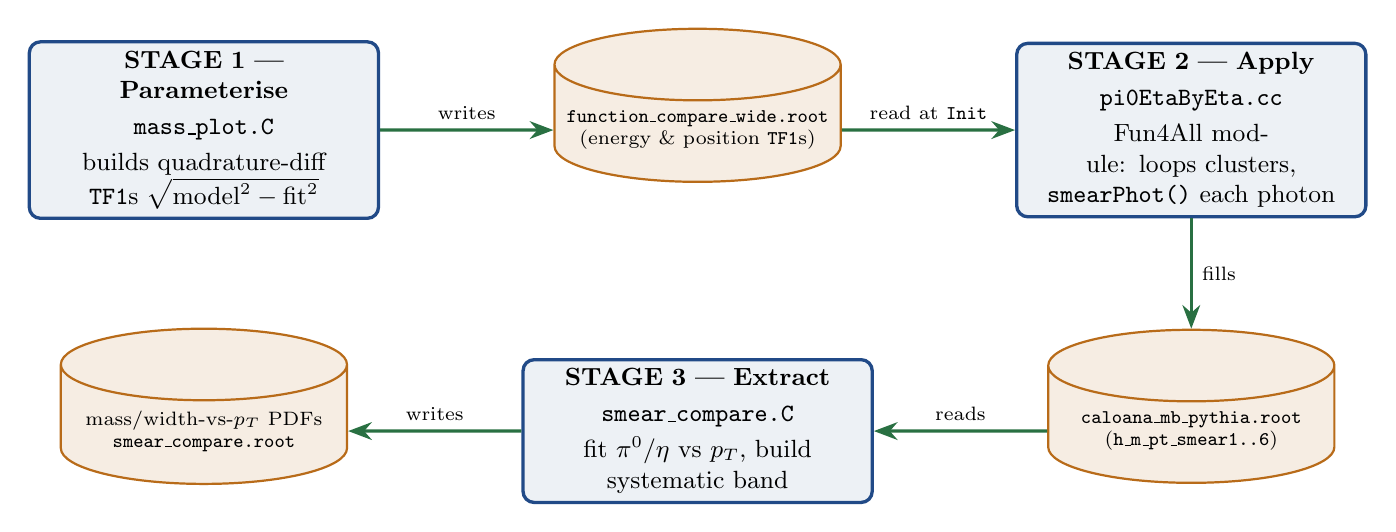
\begin{tikzpicture}[
  node distance=10mm,
  stage/.style={rectangle, rounded corners, draw=boxblue, very thick, fill=boxblue!8,
                text width=42mm, align=center, minimum height=16mm, font=\small},
  file/.style={cylinder, shape border rotate=90, aspect=0.25, draw=boxorange,
               thick, fill=boxorange!12, text width=34mm, align=center, font=\scriptsize},
  arr/.style={-{Stealth[length=3mm]}, very thick, draw=boxgreen},
]
\node[stage] (s1) {\textbf{STAGE 1 --- Parameterise}\\[2pt]\texttt{mass\_plot.C}\\[2pt]
  builds quadrature-diff \texttt{TF1}s $\sqrt{\text{model}^2-\text{fit}^2}$};
\node[file, right=22mm of s1] (f1) {\texttt{function\_compare\_wide.root}\\ (energy \& position \texttt{TF1}s)};
\node[stage, right=22mm of f1] (s2) {\textbf{STAGE 2 --- Apply}\\[2pt]\texttt{pi0EtaByEta.cc}\\[2pt]
  Fun4All module: loops clusters, \texttt{smearPhot()} each photon};

\node[file, below=14mm of s2] (f2) {\texttt{caloana\_mb\_pythia.root}\\ (\texttt{h\_m\_pt\_smear1..6})};
\node[stage, left=22mm of f2] (s3) {\textbf{STAGE 3 --- Extract}\\[2pt]\texttt{smear\_compare.C}\\[2pt]
  fit $\pi^0/\eta$ vs $p_T$, build systematic band};
\node[file, left=22mm of s3] (f3) {mass/width-vs-$p_T$ PDFs\\ \texttt{smear\_compare.root}};

\draw[arr] (s1) -- node[above,font=\scriptsize]{writes} (f1);
\draw[arr] (f1) -- node[above,font=\scriptsize]{read at \texttt{Init}} (s2);
\draw[arr] (s2) -- node[right,font=\scriptsize]{fills} (f2);
\draw[arr] (f2) -- node[above,font=\scriptsize]{reads} (s3);
\draw[arr] (s3) -- node[above,font=\scriptsize]{writes} (f3);
\end{tikzpicture}
\caption{The production smearing chain. Stage~1 derives the per-energy smearing
widths and writes them as \texttt{TF1}s. Stage~2 (the engine this document focuses on)
reads that file at \texttt{Init} and applies the smear photon-by-photon during
reconstruction. Stage~3 fits the smeared meson peaks and forms the smearing
systematic band.}
\end{figure}

\begin{description}[leftmargin=1.2em,style=nextline]
\item[Stage 1 --- \texttt{mass\_plot.C}] From data-vs-MC resolution models and the
  fitted resolution, it builds the quadrature-difference \texttt{TF1}s of
  Eq.~\eqref{eq:quaddiff} for \emph{both} energy and position, and writes them
  (names like \texttt{f\_energy\_difference\_global\_minimum},
  \texttt{f\_energy\_difference\_cE\_0p08}, \texttt{f\_energy\_difference\_cE\_0p05})
  into \texttt{function\_compare\_wide.root}.
\item[Stage 2 --- \texttt{pi0EtaByEta.cc}] The production smearing \emph{engine}
  --- a \texttt{Fun4All SubsysReco} module. It reads the \texttt{TF1}s once at
  \texttt{Init}, then in the event loop smears every photon pair and fills the
  \texttt{h\_m\_pt\_smear} histograms. Detailed in Sec.~\ref{sec:engine}.
\item[Stage 3 --- \texttt{smear\_compare.C}] Reads the smeared histograms
  (\texttt{h\_m\_pt\_smear12/13/14} A/$\sqrt{E}$ variations), fits $\pi^0$ and
  $\eta$ peaks vs $p_T$ with a \texttt{MesonFitter}, and produces the mass-scale
  and width comparison plus the max$-$min systematic band.
\end{description}

%======================================================================
\section{The engine in detail: \texttt{pi0EtaByEta.cc}}
\label{sec:engine}
%======================================================================
This is a standard sPHENIX \texttt{Fun4All} reconstruction module with the usual
life cycle: \texttt{Init()} (book histograms, load parameters) $\to$
\texttt{process\_event()} (per-event work) $\to$ \texttt{End()} (write file).
The smearing touches three of these places.

\begin{figure}[h]
\centering
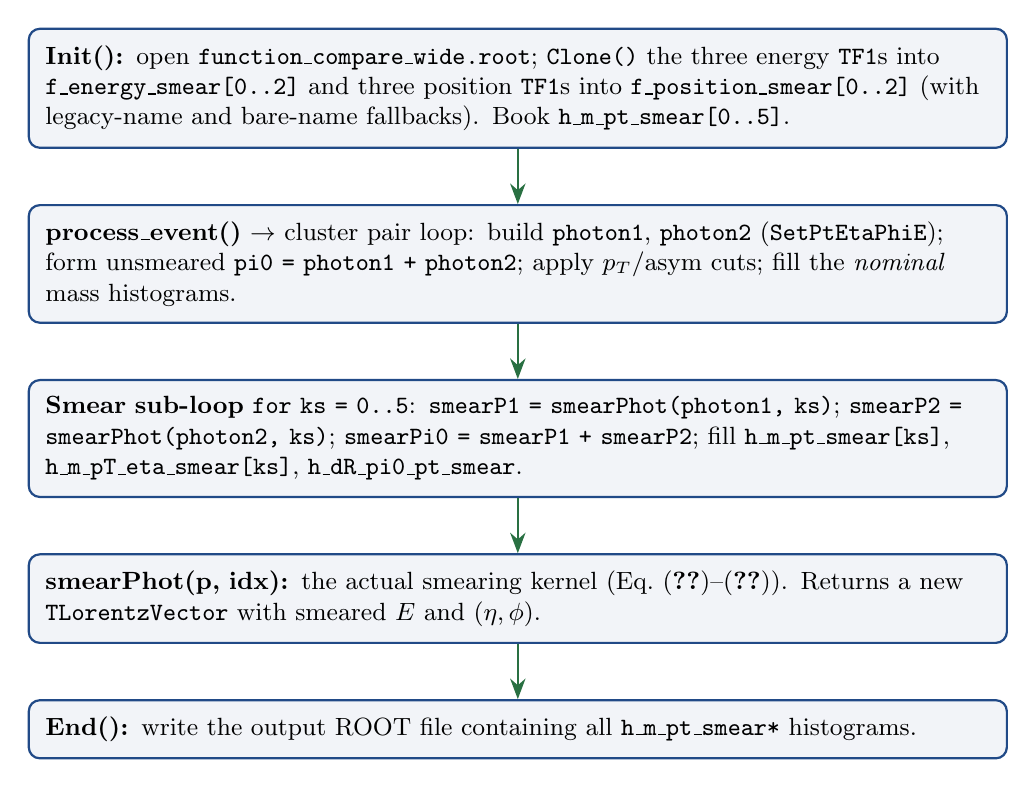
\begin{tikzpicture}[
  node distance=7mm,
  box/.style={rectangle, rounded corners, draw=boxblue, thick, fill=boxblue!6,
              text width=120mm, align=left, font=\small, inner sep=6pt},
  lab/.style={font=\bfseries\footnotesize\color{boxblue}},
  arr/.style={-{Stealth[length=2.6mm]}, thick, draw=boxgreen},
]
\node[box] (init) {\textbf{Init():} open \texttt{function\_compare\_wide.root};
  \texttt{Clone()} the three energy \texttt{TF1}s into \texttt{f\_energy\_smear[0..2]}
  and three position \texttt{TF1}s into \texttt{f\_position\_smear[0..2]} (with
  legacy-name and bare-name fallbacks). Book \texttt{h\_m\_pt\_smear[0..5]}.};
\node[box, below=of init] (loop) {\textbf{process\_event()} $\to$ cluster pair loop:
  build \texttt{photon1}, \texttt{photon2} (\texttt{SetPtEtaPhiE}); form
  unsmeared \texttt{pi0 = photon1 + photon2}; apply $p_T$/asym cuts; fill the
  \emph{nominal} mass histograms.};
\node[box, below=of loop] (sloop) {\textbf{Smear sub-loop} \texttt{for ks = 0..5}:
  \texttt{smearP1 = smearPhot(photon1, ks)};
  \texttt{smearP2 = smearPhot(photon2, ks)};
  \texttt{smearPi0 = smearP1 + smearP2};
  fill \texttt{h\_m\_pt\_smear[ks]}, \texttt{h\_m\_pT\_eta\_smear[ks]},
  \texttt{h\_dR\_pi0\_pt\_smear}.};
\node[box, below=of sloop] (sp) {\textbf{smearPhot(p, idx):} the actual smearing
  kernel (Eq.~\eqref{eq:reso}--\eqref{eq:smear}). Returns a new
  \texttt{TLorentzVector} with smeared $E$ and $(\eta,\phi)$.};
\node[box, below=of sp] (end) {\textbf{End():} write the output ROOT file
  containing all \texttt{h\_m\_pt\_smear*} histograms.};
\draw[arr] (init) -- (loop);
\draw[arr] (loop) -- (sloop);
\draw[arr] (sloop) -- (sp);
\draw[arr] (sp) -- (end);
\end{tikzpicture}
\caption{Control flow inside the production engine. The smear functions are loaded
\emph{once} at \texttt{Init} and \texttt{Eval}'d \emph{per photon} inside the event
loop.}
\end{figure}

\subsection{Loading the smear curves (\texttt{Init}, around line 206)}
The module hard-codes the parameter-file path and clones the \texttt{TF1}s into
member arrays. The fallbacks let it survive renamed/older files.
\begin{lstlisting}[firstnumber=206]
const std::string kSmearParFile =
  "/sphenix/u/bseidlitz/work/emcPerf/macros/figMaker/output/function_compare_wide.root";
TFile* smear_fin = TFile::Open(kSmearParFile.c_str(), "READ");
// for k = 0..2: get f_energy_difference_<model>, else legacy g_..., else bare name
//   f_energy_smear[k]   = (TF1*) fe->Clone(...);
//   f_position_smear[k] = (TF1*) fp->Clone(...);
\end{lstlisting}
The three indices $k=0,1,2$ correspond to the three resolution \emph{models}:
\emph{global-minimum}, $c_E=0.08$, and $c_E=0.05$.

\subsection{Booking the smeared histograms (\texttt{Init}, line 159)}
\begin{lstlisting}[firstnumber=159]
h_m_pt_smear[i]     = new TH2F(Form("h_m_pt_smear%d", i+1),     "", 500,0,1.0, 80,0,20);
h_m_pT_eta_smear[i] = new TH3F(Form("h_m_pT_eta_smear%d", i+1), "", 500,0,1.0, 80,0,20, 96,0,96);
\end{lstlisting}
Six histograms (mass $\times$ $p_T$, and mass $\times p_T\times i\eta$) --- one per
smear index. Mass axis 0--1 GeV, $p_T$ axis 0--20 GeV.

\subsection{Applying the smear in the event loop (line 738)}
For every accepted cluster pair, all six smearing variations are run and filled:
\begin{lstlisting}[firstnumber=738]
for (int ks = 0; ks < 6; ++ks) {
  TLorentzVector smearP1  = smearPhot(photon1, ks);
  TLorentzVector smearP2  = smearPhot(photon2, ks);
  TLorentzVector smearPi0 = smearP1 + smearP2;
  h_m_pt_smear[ks]->Fill(smearPi0.M(), smearPi0.Pt(), eventWeight);
  h_m_pT_eta_smear[ks]->Fill(smearPi0.M(), smearPi0.Pt(), (double)lt_eta, eventWeight);
  h_dR_pi0_pt_smear->Fill(smearP1.DeltaR(smearP2), smearPi0.Pt(), eventWeight);
}
\end{lstlisting}

\subsection{The smearing kernel: \texttt{smearPhot()} (line 863)}
This is the heart of the system. The 6 indices decode as \textbf{3 models $\times$ 2}
(with / without an extra $0.08$ constant term):
\begin{lstlisting}[firstnumber=863]
TLorentzVector pi0EtaByEta::smearPhot(TLorentzVector p, int smear_idx) {
  if (smear_idx < 0 || smear_idx > 5) smear_idx = 0;
  const int  base_smear_idx  = smear_idx % 3;   // which of 3 models
  const bool add_extra_const = (smear_idx >= 3);// 3..5 add an 0.08 const term

  const float E = p.E();
  if (E <= 0.f) return p;

  float E_res = 0.08f;     // fallbacks if TF1 missing/invalid
  float P_res = 0.0001f;

  if (f_energy_smear[base_smear_idx]) {
    double s = f_energy_smear[base_smear_idx]->Eval(E);   // sigma_extra(E)
    if (std::isfinite(s) && s > 0.0) E_res = (float)s;
  }
  if (add_extra_const)
    E_res = std::sqrt(0.08f*0.08f + E_res*E_res);          // quadrature extra const

  if (f_position_smear[base_smear_idx]) {
    double s = f_position_smear[base_smear_idx]->Eval(E);  // sigma_psi(E)
    if (std::isfinite(s) && s > 0.0) P_res = (float)s;
  }

  float Efac     = rnd->Gaus(1.0f, E_res);   // MULTIPLICATIVE energy smear
  float Pfac_phi = rnd->Gaus(0.0f, P_res);   // ADDITIVE angle smear
  float Pfac_eta = rnd->Gaus(0.0f, P_res);
  if (Efac < 0.f) Efac = 0.f;

  float eta_s = p.Eta() + Pfac_eta;
  float phi_s = p.Phi() + Pfac_phi;          // wrapped to (-pi, pi]
  const float E_s = E * Efac;
  TLorentzVector sp;
  sp.SetPtEtaPhiE(E_s/std::cosh(eta_s), eta_s, phi_s, E_s);
  return sp;
}
\end{lstlisting}

\noindent\textbf{Reading this in plain English:}
\begin{enumerate}[nosep]
  \item Pick the model ($\texttt{idx}\bmod 3$) and decide whether to add the extra
        $0.08$ constant ($\texttt{idx}\ge3$).
  \item Evaluate the stored energy-smear \texttt{TF1} at this photon's $E$ to get
        $\sigma_{\text{extra}}(E)$ (Eq.~\eqref{eq:quaddiff}); optionally fold in
        $\sqrt{0.08^2+\sigma^2}$.
  \item Evaluate the position-smear \texttt{TF1} to get the angular width
        $\sigma_\psi(E)$.
  \item \textbf{Energy} is smeared \emph{multiplicatively}: $E\to E\cdot
        \mathcal{N}(1,\sigma_{\text{extra}})$ (clamped $\ge0$).
  \item \textbf{Direction} is smeared \emph{additively}: $\eta\to\eta+\mathcal{N}(0,\sigma_\psi)$,
        $\phi\to\phi+\mathcal{N}(0,\sigma_\psi)$ (with $\phi$ wrapped).
  \item Rebuild and return a \texttt{TLorentzVector} from the smeared
        $(E_s,\eta_s,\phi_s)$.
\end{enumerate}

\begin{figure}[h]
\centering
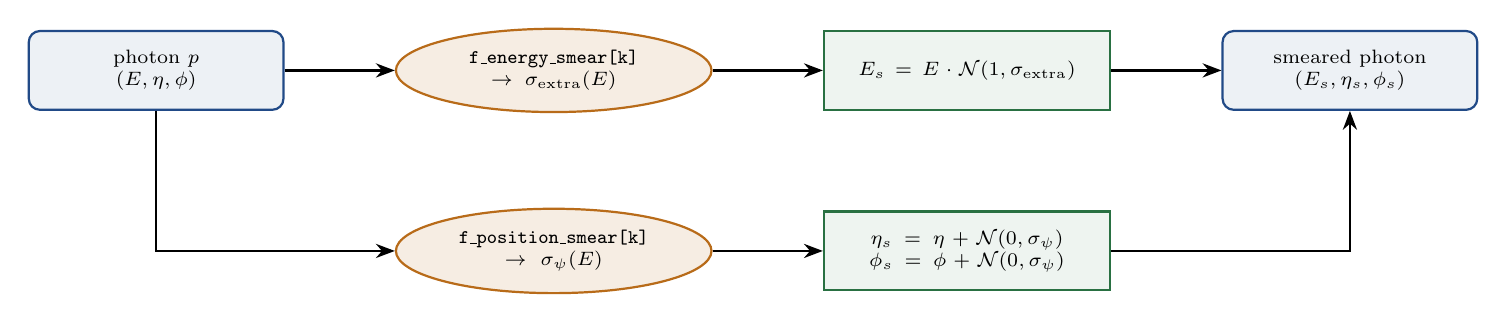
\begin{tikzpicture}[
  node distance=6mm and 14mm,
  io/.style={rectangle, rounded corners, draw=boxblue, thick, fill=boxblue!8,
             text width=30mm, align=center, font=\scriptsize, minimum height=10mm},
  op/.style={rectangle, draw=boxgreen, thick, fill=boxgreen!8,
             text width=34mm, align=center, font=\scriptsize, minimum height=10mm},
  tf/.style={ellipse, draw=boxorange, thick, fill=boxorange!12,
             text width=26mm, align=center, font=\scriptsize},
  arr/.style={-{Stealth[length=2.4mm]}, thick},
]
\node[io] (p) {photon $p$\\ $(E,\eta,\phi)$};
\node[tf, right=of p] (te) {\texttt{f\_energy\_smear[k]}\\$\to\sigma_{\text{extra}}(E)$};
\node[op, right=of te] (es) {$E_s=E\cdot\mathcal{N}(1,\sigma_{\text{extra}})$};
\node[tf, below=12mm of te] (tp) {\texttt{f\_position\_smear[k]}\\$\to\sigma_\psi(E)$};
\node[op, right=of tp] (ps) {$\eta_s=\eta+\mathcal{N}(0,\sigma_\psi)$\\$\phi_s=\phi+\mathcal{N}(0,\sigma_\psi)$};
\node[io, right=of es] (out) {smeared photon\\ $(E_s,\eta_s,\phi_s)$};
\draw[arr] (p) -- (te);
\draw[arr] (te) -- (es);
\draw[arr] (p) |- (tp);
\draw[arr] (tp) -- (ps);
\draw[arr] (es) -- (out);
\draw[arr] (ps) -| (out);
\end{tikzpicture}
\caption{Inside \texttt{smearPhot()}: energy is multiplied by a Gaussian centred at
1 (width from the energy \texttt{TF1}); the two angles are shifted by Gaussians
centred at 0 (width from the position \texttt{TF1}).}
\end{figure}

\subsection{Decoding the six smear indices}
\begin{table}[h]
\centering\small
\begin{tabular}{ccll}
\toprule
\texttt{smear\_idx} & \texttt{base=idx\%3} & resolution model & extra $0.08$ const? \\
\midrule
0 & 0 & global-minimum & no \\
1 & 1 & $c_E=0.08$      & no \\
2 & 2 & $c_E=0.05$      & no \\
3 & 0 & global-minimum & yes ($\sqrt{0.08^2+\sigma^2}$) \\
4 & 1 & $c_E=0.08$      & yes \\
5 & 2 & $c_E=0.05$      & yes \\
\bottomrule
\end{tabular}
\caption{The 6 smearing variations = 3 models $\times$ \{with, without\} an extra
constant term. Running all 6 lets Stage~3 build a systematic band by taking the
spread across variations.}
\end{table}

%======================================================================
\section{Where \texttt{CaloCalibEmc\_Pi0} fits in}
%======================================================================
\texttt{CaloCalibEmc\_Pi0} (\texttt{.cc/.h}) is the \emph{calibration} sibling
module driven by the macro \texttt{macro/Fun4All\_G4\_Pi0\_Tbt.C}. It is a
\texttt{SubsysReco} that loops clusters, builds $\pi^0$ candidates, and fits the
mass tower-by-tower / $\eta$-by-$\eta$ to derive the EMCal energy-scale calibration
constants (default target mass \texttt{0.152} GeV ``to match sim''). It is the
\emph{energy-scale} half of the data/MC matching; \texttt{pi0EtaByEta} is the
\emph{resolution} half. Together they implement the two knobs the calibration talks
turn: the scale $E_{\text{scale}}=f(E)\times0.998$ and the resolution smearing of
Eq.~\eqref{eq:reso}. The build is autotools-based
(\texttt{autogen.sh}\,$\to$\,\texttt{configure}\,$\to$\,\texttt{make install});
jobs are launched through the \texttt{Fun4All} macro plus \texttt{run\_f4a.csh} and
Condor.

%======================================================================
\section{Standalone toy cross-checks (not the production result)}
%======================================================================
Two self-contained ROOT macros validate the concept independently:
\begin{description}[leftmargin=1.2em,style=nextline]
\item[\texttt{eta\_decay\_simulation\_with\_smearing.C}] A pure toy
  $\eta\to\gamma\gamma$ generator: throw $\eta$ with a $p_T^{-4}$ spectrum, decay
  isotropically, boost to the lab, smear each photon by
  $1+\mathcal{N}(0,\sqrt{c^2+a^2/E})$ with $a=0.15,\,c=0.12$, and re-form
  $M_{\gamma\gamma}$. Demonstrates how a chosen resolution maps onto the
  reconstructed mass peak and width.
\item[\texttt{resolutionsim.C}] A toy \emph{unfolding-bias} study: for several
  (MC-reso, data-reso) pairs it trains a \texttt{RooUnfold} response from a smeared
  spectrum, unfolds a ``data'' pass smeared differently, and plots the residual
  bias --- quantifying how a data/MC resolution \emph{mismatch} propagates through
  Bayesian unfolding.
\end{description}

%======================================================================
\section{How to run the chain (summary)}
%======================================================================
\begin{enumerate}[nosep]
  \item \textbf{Build once:} \texttt{./autogen.sh \&\& ./configure --prefix=\$MYINSTALL \&\& make install}
  \item \textbf{Stage 1:} \texttt{root -l -b -q 'mass\_plot.C'} $\Rightarrow$ \texttt{function\_compare\_wide.root}
  \item \textbf{Stage 2:} \texttt{root -l -b -q 'Fun4All\_G4\_Pi0\_Tbt.C(...)'} (or \texttt{run\_f4a.csh}+Condor) $\Rightarrow$ \texttt{caloana\_mb\_pythia.root}
  \item \textbf{Stage 3:} \texttt{root -l -b -q 'smear\_compare.C'} $\Rightarrow$ mass/width-vs-$p_T$ PDFs
\end{enumerate}

%======================================================================
\section*{One-line dependency map}
\addcontentsline{toc}{section}{One-line dependency map}
%======================================================================
\begin{center}\small\ttfamily
mass\_plot.C $\to$ function\_compare\_wide.root $\to$ (Init) pi0EtaByEta::smearPhot()
$\to$ h\_m\_pt\_smear1..6 $\to$ smear\_compare.C + MesonFitter $\to$ mass/width vs $p_T$
\end{center}

%======================================================================
\section*{Key takeaways}
\addcontentsline{toc}{section}{Key takeaways}
%======================================================================
\begin{itemize}[nosep]
  \item The smear ``parameters'' are the three terms $(p_0,p_1,p_2)$ of
        Eq.~\eqref{eq:reso}; smearing widens MC by the \emph{quadrature difference}
        to data (Eq.~\eqref{eq:quaddiff}).
  \item Energy smear is \emph{multiplicative} ($\mathcal{N}(1,\sigma)$); position
        smear is \emph{additive} ($\mathcal{N}(0,\sigma_\psi)$ on $\eta$ and $\phi$).
  \item The smearing widths live in a ROOT \texttt{TF1} file produced offline; the
        engine just \texttt{Eval}s them per photon. \emph{The file is the interface
        between stages.}
  \item Six smear indices = 3 resolution models $\times$ \{with/without an extra
        0.08 constant\}; the spread across them feeds the systematic band.
  \item \texttt{pi0EtaByEta} handles \emph{resolution}; \texttt{CaloCalibEmc\_Pi0}
        handles \emph{energy scale}; together they match MC to Run-24 data.
\end{itemize}

\end{document}
